% Options for packages loaded elsewhere
\PassOptionsToPackage{unicode}{hyperref}
\PassOptionsToPackage{hyphens}{url}
\PassOptionsToPackage{dvipsnames,svgnames,x11names}{xcolor}
%
\documentclass[
]{article}
\usepackage{amsmath,amssymb}
\usepackage{iftex}
\ifPDFTeX
  \usepackage[T1]{fontenc}
  \usepackage[utf8]{inputenc}
  \usepackage{textcomp} % provide euro and other symbols
\else % if luatex or xetex
  \usepackage{unicode-math} % this also loads fontspec
  \defaultfontfeatures{Scale=MatchLowercase}
  \defaultfontfeatures[\rmfamily]{Ligatures=TeX,Scale=1}
\fi
\usepackage{lmodern}
\ifPDFTeX\else
  % xetex/luatex font selection
\fi
% Use upquote if available, for straight quotes in verbatim environments
\IfFileExists{upquote.sty}{\usepackage{upquote}}{}
\IfFileExists{microtype.sty}{% use microtype if available
  \usepackage[]{microtype}
  \UseMicrotypeSet[protrusion]{basicmath} % disable protrusion for tt fonts
}{}
\makeatletter
\@ifundefined{KOMAClassName}{% if non-KOMA class
  \IfFileExists{parskip.sty}{%
    \usepackage{parskip}
  }{% else
    \setlength{\parindent}{0pt}
    \setlength{\parskip}{6pt plus 2pt minus 1pt}}
}{% if KOMA class
  \KOMAoptions{parskip=half}}
\makeatother
\usepackage{xcolor}
\usepackage[margin=1in]{geometry}
\usepackage{color}
\usepackage{fancyvrb}
\newcommand{\VerbBar}{|}
\newcommand{\VERB}{\Verb[commandchars=\\\{\}]}
\DefineVerbatimEnvironment{Highlighting}{Verbatim}{commandchars=\\\{\}}
% Add ',fontsize=\small' for more characters per line
\usepackage{framed}
\definecolor{shadecolor}{RGB}{248,248,248}
\newenvironment{Shaded}{\begin{snugshade}}{\end{snugshade}}
\newcommand{\AlertTok}[1]{\textcolor[rgb]{0.94,0.16,0.16}{#1}}
\newcommand{\AnnotationTok}[1]{\textcolor[rgb]{0.56,0.35,0.01}{\textbf{\textit{#1}}}}
\newcommand{\AttributeTok}[1]{\textcolor[rgb]{0.13,0.29,0.53}{#1}}
\newcommand{\BaseNTok}[1]{\textcolor[rgb]{0.00,0.00,0.81}{#1}}
\newcommand{\BuiltInTok}[1]{#1}
\newcommand{\CharTok}[1]{\textcolor[rgb]{0.31,0.60,0.02}{#1}}
\newcommand{\CommentTok}[1]{\textcolor[rgb]{0.56,0.35,0.01}{\textit{#1}}}
\newcommand{\CommentVarTok}[1]{\textcolor[rgb]{0.56,0.35,0.01}{\textbf{\textit{#1}}}}
\newcommand{\ConstantTok}[1]{\textcolor[rgb]{0.56,0.35,0.01}{#1}}
\newcommand{\ControlFlowTok}[1]{\textcolor[rgb]{0.13,0.29,0.53}{\textbf{#1}}}
\newcommand{\DataTypeTok}[1]{\textcolor[rgb]{0.13,0.29,0.53}{#1}}
\newcommand{\DecValTok}[1]{\textcolor[rgb]{0.00,0.00,0.81}{#1}}
\newcommand{\DocumentationTok}[1]{\textcolor[rgb]{0.56,0.35,0.01}{\textbf{\textit{#1}}}}
\newcommand{\ErrorTok}[1]{\textcolor[rgb]{0.64,0.00,0.00}{\textbf{#1}}}
\newcommand{\ExtensionTok}[1]{#1}
\newcommand{\FloatTok}[1]{\textcolor[rgb]{0.00,0.00,0.81}{#1}}
\newcommand{\FunctionTok}[1]{\textcolor[rgb]{0.13,0.29,0.53}{\textbf{#1}}}
\newcommand{\ImportTok}[1]{#1}
\newcommand{\InformationTok}[1]{\textcolor[rgb]{0.56,0.35,0.01}{\textbf{\textit{#1}}}}
\newcommand{\KeywordTok}[1]{\textcolor[rgb]{0.13,0.29,0.53}{\textbf{#1}}}
\newcommand{\NormalTok}[1]{#1}
\newcommand{\OperatorTok}[1]{\textcolor[rgb]{0.81,0.36,0.00}{\textbf{#1}}}
\newcommand{\OtherTok}[1]{\textcolor[rgb]{0.56,0.35,0.01}{#1}}
\newcommand{\PreprocessorTok}[1]{\textcolor[rgb]{0.56,0.35,0.01}{\textit{#1}}}
\newcommand{\RegionMarkerTok}[1]{#1}
\newcommand{\SpecialCharTok}[1]{\textcolor[rgb]{0.81,0.36,0.00}{\textbf{#1}}}
\newcommand{\SpecialStringTok}[1]{\textcolor[rgb]{0.31,0.60,0.02}{#1}}
\newcommand{\StringTok}[1]{\textcolor[rgb]{0.31,0.60,0.02}{#1}}
\newcommand{\VariableTok}[1]{\textcolor[rgb]{0.00,0.00,0.00}{#1}}
\newcommand{\VerbatimStringTok}[1]{\textcolor[rgb]{0.31,0.60,0.02}{#1}}
\newcommand{\WarningTok}[1]{\textcolor[rgb]{0.56,0.35,0.01}{\textbf{\textit{#1}}}}
\usepackage{graphicx}
\makeatletter
\def\maxwidth{\ifdim\Gin@nat@width>\linewidth\linewidth\else\Gin@nat@width\fi}
\def\maxheight{\ifdim\Gin@nat@height>\textheight\textheight\else\Gin@nat@height\fi}
\makeatother
% Scale images if necessary, so that they will not overflow the page
% margins by default, and it is still possible to overwrite the defaults
% using explicit options in \includegraphics[width, height, ...]{}
\setkeys{Gin}{width=\maxwidth,height=\maxheight,keepaspectratio}
% Set default figure placement to htbp
\makeatletter
\def\fps@figure{htbp}
\makeatother
\ifLuaTeX
  \usepackage{luacolor}
  \usepackage[soul]{lua-ul}
\else
  \usepackage{soul}
\fi
\setlength{\emergencystretch}{3em} % prevent overfull lines
\providecommand{\tightlist}{%
  \setlength{\itemsep}{0pt}\setlength{\parskip}{0pt}}
\setcounter{secnumdepth}{-\maxdimen} % remove section numbering
% definitions for citeproc citations
\NewDocumentCommand\citeproctext{}{}
\NewDocumentCommand\citeproc{mm}{%
  \begingroup\def\citeproctext{#2}\cite{#1}\endgroup}
\makeatletter
 % allow citations to break across lines
 \let\@cite@ofmt\@firstofone
 % avoid brackets around text for \cite:
 \def\@biblabel#1{}
 \def\@cite#1#2{{#1\if@tempswa , #2\fi}}
\makeatother
\newlength{\cslhangindent}
\setlength{\cslhangindent}{1.5em}
\newlength{\csllabelwidth}
\setlength{\csllabelwidth}{3em}
\newenvironment{CSLReferences}[2] % #1 hanging-indent, #2 entry-spacing
 {\begin{list}{}{%
  \setlength{\itemindent}{0pt}
  \setlength{\leftmargin}{0pt}
  \setlength{\parsep}{0pt}
  % turn on hanging indent if param 1 is 1
  \ifodd #1
   \setlength{\leftmargin}{\cslhangindent}
   \setlength{\itemindent}{-1\cslhangindent}
  \fi
  % set entry spacing
  \setlength{\itemsep}{#2\baselineskip}}}
 {\end{list}}
\usepackage{calc}
\newcommand{\CSLBlock}[1]{\hfill\break\parbox[t]{\linewidth}{\strut\ignorespaces#1\strut}}
\newcommand{\CSLLeftMargin}[1]{\parbox[t]{\csllabelwidth}{\strut#1\strut}}
\newcommand{\CSLRightInline}[1]{\parbox[t]{\linewidth - \csllabelwidth}{\strut#1\strut}}
\newcommand{\CSLIndent}[1]{\hspace{\cslhangindent}#1}
\ifLuaTeX
  \usepackage{selnolig}  % disable illegal ligatures
\fi
\usepackage{bookmark}
\IfFileExists{xurl.sty}{\usepackage{xurl}}{} % add URL line breaks if available
\urlstyle{same}
\hypersetup{
  pdftitle={R Markdown Tutorial},
  pdfauthor={Ruben Bach and Christoph Kern},
  colorlinks=true,
  linkcolor={blue},
  filecolor={Maroon},
  citecolor={Blue},
  urlcolor={Blue},
  pdfcreator={LaTeX via pandoc}}

\title{R Markdown Tutorial}
\author{Ruben Bach and Christoph Kern}
\date{2024-09-11}

\begin{document}
\maketitle

{
\hypersetup{linkcolor=}
\setcounter{tocdepth}{2}
\tableofcontents
}
\section{R Markdown}\label{r-markdown}

This is an R Markdown document. Markdown is a simple formatting syntax
for authoring HTML, PDF, and MS Word documents. For more details on
using R Markdown see \url{http://rmarkdown.rstudio.com}.

When you click the \textbf{Knit} button a document will be generated
that includes both content as well as the output of any embedded R code
chunks within the document. You can embed an R code chunk like this:

\begin{Shaded}
\begin{Highlighting}[]
\FunctionTok{summary}\NormalTok{(cars)}
\end{Highlighting}
\end{Shaded}

\begin{verbatim}
##      speed           dist       
##  Min.   : 4.0   Min.   :  2.00  
##  1st Qu.:12.0   1st Qu.: 26.00  
##  Median :15.0   Median : 36.00  
##  Mean   :15.4   Mean   : 42.98  
##  3rd Qu.:19.0   3rd Qu.: 56.00  
##  Max.   :25.0   Max.   :120.00
\end{verbatim}

Same Code, but results only.

\begin{verbatim}
##      speed           dist       
##  Min.   : 4.0   Min.   :  2.00  
##  1st Qu.:12.0   1st Qu.: 26.00  
##  Median :15.0   Median : 36.00  
##  Mean   :15.4   Mean   : 42.98  
##  3rd Qu.:19.0   3rd Qu.: 56.00  
##  Max.   :25.0   Max.   :120.00
\end{verbatim}

Still same code but this time code only and no results!

\begin{Shaded}
\begin{Highlighting}[]
\FunctionTok{summary}\NormalTok{(cars)}
\end{Highlighting}
\end{Shaded}

Data tables can be formatted in different styles.

\begin{Shaded}
\begin{Highlighting}[]
\NormalTok{cars[}\DecValTok{1}\SpecialCharTok{:}\DecValTok{5}\NormalTok{, ]}
\end{Highlighting}
\end{Shaded}

\begin{verbatim}
##   speed dist
## 1     4    2
## 2     4   10
## 3     7    4
## 4     7   22
## 5     8   16
\end{verbatim}

\subsection{Including Plots}\label{including-plots}

You can also embed plots, for example:

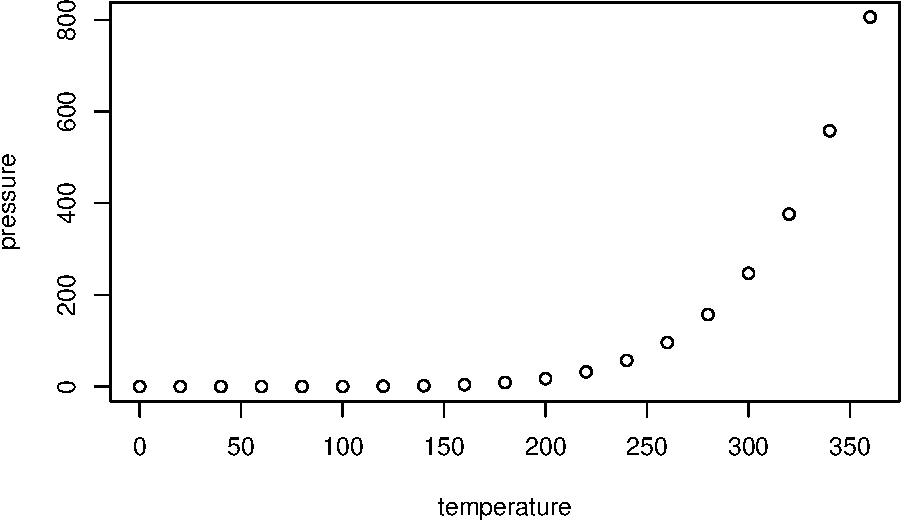
\includegraphics{03-RMarkdown_files/figure-latex/pressure-1.pdf}

For headers, use \#, \#\#, \#\#\#, \#\#\#\#, \#\#\#\#\#, \#\#\#\#\#\# t

\subsection{A large header}\label{a-large-header}

\subsubsection{\texorpdfstring{A slightly smaller header with a
\textbf{bold} word (two
asterisks)}{A slightly smaller header with a bold word (two asterisks)}}\label{a-slightly-smaller-header-with-a-bold-word-two-asterisks}

For \emph{italic} font use one asterisk. We can also \st{cross out}
words!\\
Two begin a new line, add two spaces to the end of a line.\\
A new line starts!

\section{Citations}\label{citations}

Seminal work on propensity score
(\citeproc{ref-rosenbaum1983central}{Rosenbaum and Rubin 1983}).\\
Year cited without author (\citeproc{ref-rosenbaum1983central}{1983}).\\
Rosenbaum and Rubin (\citeproc{ref-rosenbaum1983central}{1983}) cited in
line.

\section{Installing scripts}\label{installing-scripts}

\subsection{Installing packages}\label{installing-packages}

We often need to include the repository from where a package should be
installed. Also, it is good practice to check whether a required package
is already installed and then install it only if it isn't.

\begin{Shaded}
\begin{Highlighting}[]
\ControlFlowTok{if}\NormalTok{ (}\SpecialCharTok{!}\FunctionTok{require}\NormalTok{(}\StringTok{\textquotesingle{}MASS\textquotesingle{}}\NormalTok{)) }\FunctionTok{install.packages}\NormalTok{(}\StringTok{\textquotesingle{}MASS\textquotesingle{}}\NormalTok{, }\AttributeTok{repos =} \StringTok{"http://cran.us.r{-}project.org"}\NormalTok{)}
\FunctionTok{library}\NormalTok{(}\StringTok{\textquotesingle{}MASS\textquotesingle{}}\NormalTok{) }
\ControlFlowTok{if}\NormalTok{ (}\SpecialCharTok{!}\FunctionTok{require}\NormalTok{(}\StringTok{\textquotesingle{}ggplot2\textquotesingle{}}\NormalTok{)) }\FunctionTok{install.packages}\NormalTok{(}\StringTok{\textquotesingle{}ggplot2\textquotesingle{}}\NormalTok{, }\AttributeTok{repos =} \StringTok{"http://cran.us.r{-}project.org"}\NormalTok{)}
\FunctionTok{library}\NormalTok{(}\StringTok{\textquotesingle{}ggplot2\textquotesingle{}}\NormalTok{) }
\ControlFlowTok{if}\NormalTok{ (}\SpecialCharTok{!}\FunctionTok{require}\NormalTok{(}\StringTok{\textquotesingle{}dplyr\textquotesingle{}}\NormalTok{)) }\FunctionTok{install.packages}\NormalTok{(}\StringTok{\textquotesingle{}dplyr\textquotesingle{}}\NormalTok{, }\AttributeTok{repos =} \StringTok{"http://cran.us.r{-}project.org"}\NormalTok{)}
\FunctionTok{library}\NormalTok{(}\StringTok{\textquotesingle{}dplyr\textquotesingle{}}\NormalTok{) }
\end{Highlighting}
\end{Shaded}

\section{Example analysis}\label{example-analysis}

We estimate a linear regression model explaining the price of a diamond
by its clarity, cut, and carat. By the way, the mean of c(1:5) is 3.

\begin{Shaded}
\begin{Highlighting}[]
\NormalTok{regmod}\FloatTok{.1} \OtherTok{\textless{}{-}} \FunctionTok{lm}\NormalTok{(price }\SpecialCharTok{\textasciitilde{}}\NormalTok{ clarity }\SpecialCharTok{+}\NormalTok{ cut }\SpecialCharTok{+}\NormalTok{ carat, }\AttributeTok{data =}\NormalTok{ diamonds)}
\FunctionTok{summary}\NormalTok{(regmod}\FloatTok{.1}\NormalTok{) }
\end{Highlighting}
\end{Shaded}

\begin{verbatim}
## 
## Call:
## lm(formula = price ~ clarity + cut + carat, data = diamonds)
## 
## Residuals:
##      Min       1Q   Median       3Q      Max 
## -16842.5   -636.4   -114.3    474.8  11238.6 
## 
## Coefficients:
##              Estimate Std. Error  t value Pr(>|t|)    
## (Intercept) -3187.540     14.475 -220.208   <2e-16 ***
## clarity.L    4011.681     33.931  118.231   <2e-16 ***
## clarity.Q   -1821.922     31.870  -57.167   <2e-16 ***
## clarity.C     917.658     27.313   33.598   <2e-16 ***
## clarity^4    -430.047     21.831  -19.699   <2e-16 ***
## clarity^5     257.141     17.821   14.429   <2e-16 ***
## clarity^6      26.909     15.539    1.732   0.0833 .  
## clarity^7     186.742     13.685   13.646   <2e-16 ***
## cut.L         713.804     22.511   31.709   <2e-16 ***
## cut.Q        -334.503     19.828  -16.871   <2e-16 ***
## cut.C         188.482     17.218   10.947   <2e-16 ***
## cut^4           1.663     13.794    0.121   0.9040    
## carat        8472.026     12.615  671.584   <2e-16 ***
## ---
## Signif. codes:  0 '***' 0.001 '**' 0.01 '*' 0.05 '.' 0.1 ' ' 1
## 
## Residual standard error: 1281 on 53927 degrees of freedom
## Multiple R-squared:  0.8969, Adjusted R-squared:  0.8969 
## F-statistic: 3.911e+04 on 12 and 53927 DF,  p-value: < 2.2e-16
\end{verbatim}

\section{Parameters}\label{parameters}

\begin{Shaded}
\begin{Highlighting}[]
\FunctionTok{print}\NormalTok{(}\FunctionTok{paste}\NormalTok{(}\StringTok{"The years is "}\NormalTok{, params}\SpecialCharTok{$}\NormalTok{year))}
\end{Highlighting}
\end{Shaded}

\begin{verbatim}
## [1] "The years is  2020"
\end{verbatim}

\begin{Shaded}
\begin{Highlighting}[]
\NormalTok{regmod}\FloatTok{.2} \OtherTok{\textless{}{-}} \FunctionTok{lm}\NormalTok{(mpg }\SpecialCharTok{\textasciitilde{}}\NormalTok{ cyl }\SpecialCharTok{+}\NormalTok{ disp, }\AttributeTok{data =}\NormalTok{ params}\SpecialCharTok{$}\NormalTok{data)}
\FunctionTok{summary}\NormalTok{(regmod}\FloatTok{.2}\NormalTok{) }
\end{Highlighting}
\end{Shaded}

\begin{verbatim}
## 
## Call:
## lm(formula = mpg ~ cyl + disp, data = params$data)
## 
## Residuals:
##     Min      1Q  Median      3Q     Max 
## -4.4213 -2.1722 -0.6362  1.1899  7.0516 
## 
## Coefficients:
##             Estimate Std. Error t value Pr(>|t|)    
## (Intercept) 34.66099    2.54700  13.609 4.02e-14 ***
## cyl         -1.58728    0.71184  -2.230   0.0337 *  
## disp        -0.02058    0.01026  -2.007   0.0542 .  
## ---
## Signif. codes:  0 '***' 0.001 '**' 0.01 '*' 0.05 '.' 0.1 ' ' 1
## 
## Residual standard error: 3.055 on 29 degrees of freedom
## Multiple R-squared:  0.7596, Adjusted R-squared:  0.743 
## F-statistic: 45.81 on 2 and 29 DF,  p-value: 1.058e-09
\end{verbatim}

For a nicer look of the regression output, we can use the stargazer
package

\begin{Shaded}
\begin{Highlighting}[]
\FunctionTok{library}\NormalTok{(stargazer)}
\FunctionTok{stargazer}\NormalTok{(regmod}\FloatTok{.1}\NormalTok{,}
          \AttributeTok{title =} \StringTok{"Regression table with stargazer"}\NormalTok{,}
          \AttributeTok{label=}\StringTok{"tab1"}\NormalTok{, }
          \AttributeTok{model.numbers =} \ConstantTok{FALSE}\NormalTok{,}
          \AttributeTok{type=}\StringTok{"latex"}\NormalTok{)}
\end{Highlighting}
\end{Shaded}

\% Table created by stargazer v.5.2.3 by Marek Hlavac, Social Policy
Institute. E-mail: marek.hlavac at gmail.com \% Date and time: Wed, Sep
11, 2024 - 03:16:20 PM

\begin{table}[!htbp] \centering 
  \caption{Regression table with stargazer} 
  \label{tab1} 
\begin{tabular}{@{\extracolsep{5pt}}lc} 
\\[-1.8ex]\hline 
\hline \\[-1.8ex] 
 & \multicolumn{1}{c}{\textit{Dependent variable:}} \\ 
\cline{2-2} 
\\[-1.8ex] & price \\ 
\hline \\[-1.8ex] 
 clarity.L & 4,011.681$^{***}$ \\ 
  & (33.931) \\ 
  & \\ 
 clarity.Q & $-$1,821.922$^{***}$ \\ 
  & (31.870) \\ 
  & \\ 
 clarity.C & 917.658$^{***}$ \\ 
  & (27.313) \\ 
  & \\ 
 clarity$\hat{\mkern6mu}$4 & $-$430.047$^{***}$ \\ 
  & (21.831) \\ 
  & \\ 
 clarity$\hat{\mkern6mu}$5 & 257.141$^{***}$ \\ 
  & (17.821) \\ 
  & \\ 
 clarity$\hat{\mkern6mu}$6 & 26.909$^{*}$ \\ 
  & (15.539) \\ 
  & \\ 
 clarity$\hat{\mkern6mu}$7 & 186.742$^{***}$ \\ 
  & (13.685) \\ 
  & \\ 
 cut.L & 713.804$^{***}$ \\ 
  & (22.511) \\ 
  & \\ 
 cut.Q & $-$334.503$^{***}$ \\ 
  & (19.828) \\ 
  & \\ 
 cut.C & 188.482$^{***}$ \\ 
  & (17.218) \\ 
  & \\ 
 cut$\hat{\mkern6mu}$4 & 1.663 \\ 
  & (13.794) \\ 
  & \\ 
 carat & 8,472.026$^{***}$ \\ 
  & (12.615) \\ 
  & \\ 
 Constant & $-$3,187.540$^{***}$ \\ 
  & (14.475) \\ 
  & \\ 
\hline \\[-1.8ex] 
Observations & 53,940 \\ 
R$^{2}$ & 0.897 \\ 
Adjusted R$^{2}$ & 0.897 \\ 
Residual Std. Error & 1,280.935 (df = 53927) \\ 
F Statistic & 39,106.570$^{***}$ (df = 12; 53927) \\ 
\hline 
\hline \\[-1.8ex] 
\textit{Note:}  & \multicolumn{1}{r}{$^{*}$p$<$0.1; $^{**}$p$<$0.05; $^{***}$p$<$0.01} \\ 
\end{tabular} 
\end{table}

Simply include a references heading at the end. References will be added
automatically.

\section*{References}\label{references}
\addcontentsline{toc}{section}{References}

\phantomsection\label{refs}
\begin{CSLReferences}{1}{1}
\bibitem[\citeproctext]{ref-rosenbaum1983central}
Rosenbaum, Paul R., and Donald B. Rubin. 1983. {``The Central Role of
the Propensity Score in Observational Studies for Causal Effects.''}
\emph{Biometrika} 70(1):41--55.

\end{CSLReferences}

\end{document}
